%! TeX program = lualatex
\documentclass[12pt,a4paper]{article}

\usepackage[nil]{babel}
\usepackage{unicode-math}
\usepackage[svgnames]{xcolor}
\usepackage{lmodern}
\usepackage{graphicx}
\usepackage{wrapfig}
\usepackage{float}
\usepackage{parskip}

\babelprovide[import=el, main, onchar=ids fonts]{greek} % can also do import=el-polyton
\babelprovide[import, onchar=ids fonts]{english}

\babelfont{rm}
          [Language=Default]{Liberation Sans}
\babelfont[english]{rm}
          [Language=Default]{Liberation Sans}
\babelfont{sf}
          [Language=Default]{Liberation Sans}
\babelfont{tt}
          [Language=Default]{Liberation Sans}

%Enter Title Here
 \title{Domain-model-v0.3 \\ LibShare}
\author{\textbf{Ονόματα / ΑΜ / Έτος:} \\ Γρηγόρης Καπαδούκας / 1072484 / 4\textdegree \\ Χρήστος Μπεστητζάνος / 1072615 / 4\textdegree \\ Νικόλαος Αυγέρης / 1067508 / 5\textdegree \\ Περικλής Κοροντζής / 1072563 / 4\textdegree}

\begin{document}

\makeatletter
\begin{center}
	\LARGE{\@title} \\
	\pagebreak
    \begin{LARGE}\@author\end{LARGE} 
    \pagebreak
\end{center}

%Insert Body Here
\section{Σχήμα Domain Model}

\begin{figure}[H]
	\makebox[\textwidth]{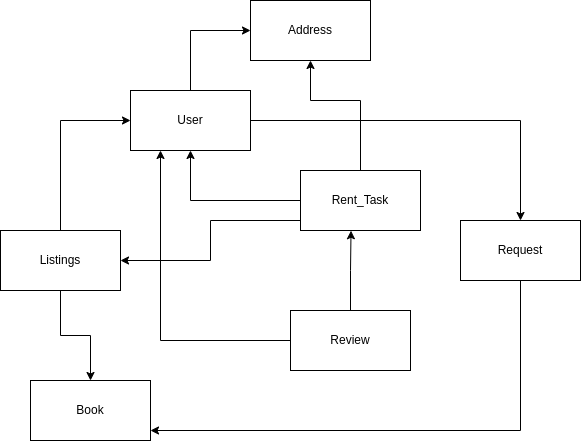
\includegraphics[width=\textwidth]{Domain model.png}}
	\caption{Σχήμα Domain Model}
	\label{Σχήμα Domain Model}
\end{figure}

\section{Σύντομη περιγραφή κλάσεων}

\subsection{Χρήστης}
Ο κάθε χρήστης που είναι εγγεγραμμένος στην εφαρμογή μαζί με τα στοιχεία του. 
%Θα περιέχει βασικές πληροφορίες όπως όνομα, ηλικία, ποσό στον λογαριασμό του κλπ.

\subsection{Διεύθυνση}
Διευθύνσεις χρηστών που έχουν αποθηκευτεί στο σύστημα. Συνδέονται με τη κλάση "Χρήστης" με σχέση συνάθροισης. Χρησιμοποιείται στην ανταλλαγή πληροφοριών μεταξύ χρηστών κατά την ώρα συναλλαγών, ώστε να μπορούν να γίνουν συναλλαγές ταχυδρομικώς.

\subsection{Πόλη}
Πόλεις στις οποίες ανήκουν οι διευθύνσεις των χρηστών. Συνδέονται με τη κλάση "Διεύθυνση" με σχέση συνάθροισης. Χρησιμοποιείται για συναλλαγές, ώστε να μπορεί το σύστημα για παράδειγμα να δείχνει μόνο βιβλία που προσφέρουν χρήστες που μένουν στην ίδια πόλη με τον χρήστη που αναζητά.

\subsection{Καταχώρηση}
Οι καταχωρήσεις χρηστών αποτελούν τις "προσφορές" που αναρτούν στην εφαρμογή με σκοπό να γίνουν αποδεκτές από άλλους χρήστες. Συνδέεται με σχέση σύνθεσης με την κλάση "Χρήστης".
.
\subsection{Προσφορά βιβλίου}
Αποτελεί τα βιβλία που προσφέρει ο χρήστης για ενοικίαση από άλλους χρήστες. Αποτελεί κλάση παιδί της κλάσης "Καταχώρηση".
%Έχει δεδομένα όπως: Ιδιοκτήτης βιβλίου (τύπου User), Βιβλίο (τύπου Book), τιμή κ.α.

\subsection{Αίτηση βιβλίου}
Αποτελεί τις αιτήσεις βιβλίων που κάνει ο χρήστης. Δηλαδή αποτελεί αιτήσεις για βιβλία που δεν προσφέρονται ήδη από άλλο χρήστη, με σκοπό ο κάποιος που έχει το βιβλίο αλλά δεν το προσφέρει να αποδεχτεί την αίτηση και να νοικιάσει το βιβλίο στον χρήστη που το ζητάει, λαμβάνοντας μια επιπλέον ανταμοιβή. Αποτελεί κλάση παιδί της κλάσης "Καταχώρηση".
%Περιέχονται δεδομένα όπως: ο χρήστης που έκανε το request (τύπου User), το βιβλίο που ψάχνει (τύπου Book), την κατάσταση της αίτησης ("Ολοκληρωμένη" ή "Ενεργή") κ.α.

\subsection{Βιβλίο}
Τα βιβλία που έχουν εισαχθεί στο σύστημα κατά την δημιουργία κάποιας καταχώρησης (είτε είναι διαθέσιμα για ενοικίαση είτε όχι). Συνδέεται με σχέση συνάθροισης με την κλάση "Καταχώρηση".
%Περιέχονται βασικές πληροφορίες των βιβλίων όπως τίτλος, συγγραφέας, είδος (πχ φαντασίας), κατηγορία (πχ νουβέλα).

\subsection{Συναλλαγή}
Από τη στιγμή που κάποιος χρήστης κάνει αίτηση ενοικίασης ενός βιβλίου ή αίτηση εκπλήρωσης αίτησης δημιουργείται μια συναλλαγή. Αυτή έχει σκοπό να καταγράφει την κατάσταση της συναλλαγής, όπως αν είναι ενεργή, ακυρωμένη ή ολοκληρωμένη. Συνδέεται με σχέση συνάθροισης με την κλάση "Χρήστης".
%Περιέχει δεδομένα όπως τον ιδιοκτήτη του βιβλίου (τύπου user), τον ενοικιαστή (τύπου user) το βιβλίο (τύπου Listing) την κατάσταση (σε τι κατάσταση βρίσκεται η διαδικασία, π.χ. "Ολοκληρωμένη", "Αναμένεται αποστολή" κ.α) και Tracking Number στη περίπτωση που γίνεται ταχυδρομική συναλλαγή.

\subsection{Αξιολόγηση}
Μετά την ολοκλήρωση κάθε συναλλαγής οι χρήστες μπορούν να εισάγουν αξιολόγηση για τον χρήστη με τον οποίο έκαναν την συναλλαγή (ιδιοκτήτη ή ενοικιαστή), μαζί με προαιρετικό σχόλιο. Αυτές οι κριτικές αποτελούν στιγμιότυπα κλάσης "Αξιολόγηση" και συνδέονται με την κλάση "Συναλλαγή" με σχέση σύνδεσης.


\subsection{Αγαπημένος Χρήστης}
Αποτελεί κλάση που καταγράφει χρήστες τους οποίους ένας χρήστης “ακολουθεί” (δηλαδή έχει προσθέσει στην λίστα αγαπημένων του). Συνδέεται με σχέση σύνθεσης με την κλάση "Χρήστης".
%Αποθηκεύεται ο χρήστης "αγαπημένος" και ο χρήστης που πρόσθεσε τον άλλον στη λίστα του.

\subsection{Ειδοποίηση}
Όταν ένας αγαπημένος χρήστης ενός άλλου χρήστη προσθέσει νέα καταχώρηση στην πλατφόρμα δημιουργείται μια ειδοποίηση για τον χρήστη, προσφέροντας έτσι τη δυνατότητα στους χρήστες να ενημερώνονται άμεσα για τις νέες καταχωρήσεις των "αγαπημένων" τους. Η ειδοποίηση αυτή είναι στιγμιότυπο της κλάσης "Ειδοποίηση", η οποία συνδέεται με σχέση σύνθεσης με την κλάση "Χρήστης".

\section{Συμμετοχή και Ρόλοι στη Συγγραφή του Κειμένου}
\begin{enumerate}
	\item \textbf{Γρηγόρης Καπαδούκας:} Author
	\item \textbf{Περικλής Κοροντζής:} Author
\end{enumerate}

\section{Αλλαγές από έκδοση σε έκδοση}

\subsection{Από έκδοση v0.1 σε έκδοση v0.2}
\begin{itemize}
    \item Σχεδίαση του Domain-model από την αρχή, μέσω του Visual Paradigm.
    \item Προσθήκη σωστών συσχετίσεων μεταξύ κλάσεων.
    \item Μετάφραση ονομάτων κλάσεων στα ελληνικά.
    \item Προσθήκη της κλάσης "Καταχώρηση" και ορισμός των "Προσφορά βιβλίου" και "Αίτηση βιβλίου" ως κλάσεις παιδιά της.
    \item Προσθήκη κλάσεων "Πόλη", "Ειδοποίηση", "Αγαπημένος χρήστης".
\end{itemize}

\subsection{Από έκδοση v0.2 σε έκδοση v0.3}
\begin{itemize}
    \item Προσθήκη στατικού μοντέλου attributes που προέκυψαν από τα Robustness Diagrams.
    \item Προσθήκη μεθόδων στις κλάσεις από το Sequence Diagram.
    \item Προσθήκη multiplicities of associations.
\end{itemize}

\end{document}
